%%%%%%%%%%%%%%%%%%%%%%%%%%%%%%%%%%%%%%%%%%%%%%%%%%%%%%%%%%%%%%%%%%%%%%%%%%%%%%%%%%%%
% Document data
%%%%%%%%%%%%%%%%%%%%%%%%%%%%%%%%%%%%%%%%%%%%%%%%%%%%%%%%%%%%%%%%%%%%%%%%%%%%%%%%%%%%
\documentclass[12pt]{article}
%%%%%%%%%%%%%%%%%%%%%%%%%%%%%%%%%%%%%%%%%%%%%%%%%%%%%%%%%%%%%%%%%%%%%%%%%%%%%%%%%%%%




%%%%%%%%%%%%%%%%%%%%%%%%%%%%%%%%%%%%%%%%%%%%%%%%%%%%%%%%%%%%%%%%%%%%%%%%%%%%%%%%%%%%
% Packages
%%%%%%%%%%%%%%%%%%%%%%%%%%%%%%%%%%%%%%%%%%%%%%%%%%%%%%%%%%%%%%%%%%%%%%%%%%%%%%%%%%%%
\usepackage{color, soul, xcolor} % Colored text and highlighting, respectively
\usepackage{tikz-cd} % For commutative diagrams
\usepackage{mathtools}
\usepackage{answers}
\usepackage{setspace}
\usepackage{graphicx}
\usepackage{enumerate}
\usepackage{multicol}
\usepackage{mathrsfs}
\usepackage[margin=1.25in]{geometry} 
\usepackage{amsmath,amsthm,amssymb}
\usepackage{marvosym,wasysym} 
\usepackage[framemethod=TikZ]{mdframed}
\usepackage{float}
\usepackage{morefloats}
%%%%%%%%%%%%%%%%%%%%%%%%%%%%%%%%%%%%%%%%%%%%%%%%%%%%%%%%%%%%%%%%%%%%%%%%%%%%%%%%%%%%




%%%%%%%%%%%%%%%%%%%%%%%%%%%%%%%%%%%%%%%%%%%%%%%%%%%%%%%%%%%%%%%%%%%%%%%%%%%%%%%%%%%%
% Shortcuts
%%%%%%%%%%%%%%%%%%%%%%%%%%%%%%%%%%%%%%%%%%%%%%%%%%%%%%%%%%%%%%%%%%%%%%%%%%%%%%%%%%%%
% Number systems
\newcommand{\N}{\mathbb{N}}
\newcommand{\Z}{\mathbb{Z}}
\newcommand{\C}{\mathbb{C}}
\newcommand{\R}{\mathbb{R}}
\newcommand{\Q}{\mathbb{Q}}
\newcommand{\field}{\mathbb{F}}
\newcommand{\linmap}{\overset{\sim}{\longrightarrow}}
\newcommand{\Hom}{\mathrm{Hom}}
\newcommand{\End}{\mathrm{End}}
\newcommand{\Aut}{\mathrm{Aut}}
\newcommand{\tspace}{T_q^pV}
\newcommand{\sign}{\mathrm{sign}}
\newcommand{\dmap}{\overset{d}{\longrightarrow}}

% Operators/functions
\newcommand{\id}{\mathrm{Id}}
\DeclareMathOperator{\sech}{sech}
\DeclareMathOperator{\csch}{csch}
\newcommand{\position}{\boldsymbol{\gamma}}
\newcommand{\velocity}{\boldsymbol{\dot{\gamma}}}
\newcommand{\action}{\mathcal{S}}
\newcommand{\lagrangian}{\mathcal{L}}
%%%%%%%%%%%%%%%%%%%%%%%%%%%%%%%%%%%%%%%%%%%%%%%%%%%%%%%%%%%%%%%%%%%%%%%%%%%%%%%%%%%%




%%%%%%%%%%%%%%%%%%%%%%%%%%%%%%%%%%%%%%%%%%%%%%%%%%%%%%%%%%%%%%%%%%%%%%%%%%%%%%%%%%%%
% Environments
%%%%%%%%%%%%%%%%%%%%%%%%%%%%%%%%%%%%%%%%%%%%%%%%%%%%%%%%%%%%%%%%%%%%%%%%%%%%%%%%%%%%
% Italic font
\newtheorem{proposition}{Proposition}[section]
\newtheorem{theorem}{Theorem}[section]
\newtheorem{lemma}{Lemma}[section]
\newtheorem{corollary}{Corollary}[section]
\newtheorem{axiom}{Axiom}[section]


% Plain font
\theoremstyle{definition}
\newtheorem{definition}{Definition}[section]
\newtheorem{definitions}{Definitions}[section]
\newtheorem{example}{Example}[section]
\newtheorem{remark}{Remark}[section]
\newtheorem{solution}{Solution}[section]
\newtheorem{problem}{Problem}[section]
\newtheorem{answer}{Answer}[section]
\newtheorem{question}{Question}[section]
\newtheorem{exercise}{Exercise}[section]
%%%%%%%%%%%%%%%%%%%%%%%%%%%%%%%%%%%%%%%%%%%%%%%%%%%%%%%%%%%%%%%%%%%%%%%%%%%%%%%%%%%%
 

%% Example
%%%%%%%%%%%%%%%%%%%%%%%%%%%%%%%%%%%%%%%%%%%%%%%%%%%%%%%%%
\newcounter{ex}[section]\setcounter{ex}{0}
\renewcommand{\theex}{\arabic{section}.\arabic{ex}}
\newenvironment{ex}[2][]{%
\refstepcounter{ex}%
\ifstrempty{#1}%
{\mdfsetup{%
frametitle={%
\tikz[baseline=(current bounding box.east),outer sep=0pt]
\node[anchor=east,rectangle,fill=green!20]
{\strut Example~\theex};}}
}%
{\mdfsetup{%
frametitle={%
\tikz[baseline=(current bounding box.east),outer sep=0pt]
\node[anchor=east,rectangle,fill=orange!20]
{\strut Example~\theex:~#1};}}%
}%
\mdfsetup{innertopmargin=5pt,linecolor=orange!20,%
linewidth=2pt,topline=true,%
frametitleaboveskip=\dimexpr-\ht\strutbox\relax
}
\begin{mdframed}[]\relax%
\label{#2}}{\end{mdframed}}

%% Def
%%%%%%%%%%%%%%%%%%%%%%%%%%%%%%%%%%%%%%%%%%%%%%%%%%%%%%%%%
\newcounter{def}[section]\setcounter{def}{0}
\renewcommand{\thedef}{\arabic{section}.\arabic{def}}
\newenvironment{df}[2][]{%
\refstepcounter{lem}%
\ifstrempty{#1}%
{\mdfsetup{%
frametitle={%
\tikz[baseline=(current bounding box.east),outer sep=0pt]
\node[anchor=east,rectangle,fill=green!20]
{\strut Definition~\thelem};}}
}%
{\mdfsetup{%
frametitle={%
\tikz[baseline=(current bounding box.east),outer sep=0pt]
\node[anchor=east,rectangle,fill=green!20]
{\strut Definition~\thetheo:~#1};}}%
}%
\mdfsetup{innertopmargin=5pt,linecolor=green!20,%
linewidth=2pt,topline=true,%
frametitleaboveskip=\dimexpr-\ht\strutbox\relax
}
\begin{mdframed}[]\relax%
\label{#2}}{\end{mdframed}}

%% Prop
%%%%%%%%%%%%%%%%%%%%%%%%%%%%%%%%%%%%%%%%%%%%%%%%%%%%%%%%%
\newcounter{prop}[section]\setcounter{prop}{0}
\renewcommand{\theprop}{\arabic{section}.\arabic{prop}}
\newenvironment{prop}[2][]{%
\refstepcounter{prop}%
\ifstrempty{#1}%
{\mdfsetup{%
frametitle={%
\tikz[baseline=(current bounding box.east),outer sep=0pt]
\node[anchor=east,rectangle,fill=red!20]
{\strut Proposition~\theprf};}}
}%
{\mdfsetup{%
frametitle={%
\tikz[baseline=(current bounding box.east),outer sep=0pt]
\node[anchor=east,rectangle,fill=red!20]
{\strut Proposition~\thetheo:~#1};}}%
}%
\mdfsetup{innertopmargin=5pt,linecolor=red!20,%
linewidth=2pt,topline=true,%
frametitleaboveskip=\dimexpr-\ht\strutbox\relax
}
\begin{mdframed}[]\relax%
\label{#2}}{\qed\end{mdframed}}

 
%%%%%%%%%%%%%%%%%%%%%%%%%%%%%%%%%%%%%%%%%%%%%%%%%%%%%%%%%%%%%%%%%%%%%%%%%%%%%%%%%%%%
% Beginning of document
%%%%%%%%%%%%%%%%%%%%%%%%%%%%%%%%%%%%%%%%%%%%%%%%%%%%%%%%%%%%%%%%%%%%%%%%%%%%%%%%%%%%
\title{The Principle of Least Action and Variational Methods}
\author{Colin Roberts}


\begin{document}
\maketitle

\setcounter{section}{-1}
\section{Introduction}
There are three main avenues for studying classical mechanics:
\begin{itemize}
    \item Newtonian,
    \item Hamiltonian,
    \item Lagrangian.
\end{itemize}
Each one of these approaches ends up being equivalent.  However, there are different reasons for wanting to use each.\\

\noindent \underline{Newton:} The original mechanical perspective.  Roughly stated, in an inertial frame, an object moves in a straight line unless acted upon by an external force. The deviation from a straight line is equal to the applied force times the reciprocal mass of the object. This gives us that the change in velocity of an object (i.e., the acceleration) must evolve by
\[
\mathbf{\ddot{x}} = \frac{\mathbf{F}}{m}.
\]

\noindent \underline{Hamilton:} Mechanical systems conserve energy.  The Hamiltonian function is the total energy function given by
\[
H=T+V,
\]
where $T$ is the kinetic energy and $V$ the potential energy.  Given this conserved energy, we can realize trajectories by solving Hamilton's equations
\[
\mathbf{\dot{x}}=\frac{\partial H}{\partial \mathbf{p}}, \quad \textrm{and} \quad \mathbf{\dot{p}} = -\frac{\partial H}{\partial \mathbf{x}}.
\]
If a particle is constrained to some manifold $M$, then the cotangent bundle $T^*M$ is the \emph{phase space} for the particle. The cotangent bundle is canonically a symplectic manifold, and tools from symplectic geometry prove useful here.

\noindent \underline{Lagrange:} Particle trajectories follow the \emph{principle of least action}. That is, particles wish to expend the least amount of energy over time as possible as it traverses from a point $a$ to a point $b$. 

We think of particles living on a manifold $M$ with position $\position$ and velocity $\velocity$.  Thus, the \emph{configuration space} for the particle is naturally the tangent bundle $TM$.  

\begin{remark}
You can obtain Hamilton's equations from the Legendre transformation of the Lagrangian formulation.  In this respect, the two are canonically equivalent.  To me, it seems that the Lagrangian perspective is more natural.
\end{remark}

\noindent \textbf{Goals for this talk:}
\begin{itemize}
    \item Determine the Lagrangian function and the associated action.
    \begin{itemize}
        \item Understand its interpretation.
        \item Consider the free energy.
        \item Look at example problems.
    \end{itemize}
    \item Define the first order variation of a functional.
    \begin{itemize}
        \item Realize Newton's laws in mechanics.
        \item Realize the Laplace equation.
    \end{itemize}
    \item Consider constricted free particles.
    \begin{itemize}
        \item The general problem statement.
        \item Riemannian geometry.
        \item The geodesic equations.
        \item The minimal surface problem.
    \end{itemize}
\end{itemize}

\section{Determining the Lagrangian and Action}

Let's say a particle (system) is to travel from a point (state) $a$ to a point (state) $b$.  This requires the particle (system) to have kinetic energy, but the particle (system) can be granted energy from a potential. (From now on, I will only say particle and point but keep in mind that we could exchange a particle for a system and a point with a state of that system.)  The analogy follows.

The particle spontaneously generating kinetic energy comes at a cost whereas the particle can happily be granted energy from a potential in its ambient environment.  For a concrete example, just imagine a particle dropped from a height $h$ above the Earth's surface. It happily takes this potential energy and makes use of it. 

\begin{df}[Lagrangian]{def: lagrangian}
We define a ``cost" function that acts on the configuration space $T\R^n$ (the tangent bundle of $\R^n$) and time $\R$ 
\[
\mathcal{L}\colon T\R^n \times \R \to \R
\]
given by
\[
\mathcal{L}(\position,\velocity,t) = T(\position,\velocity,t)-V(\position,\velocity, t).
\]
We call such $\mathcal{L}$ the \emph{Lagrangian} and, again, $T$ is the kinetic energy, and $V$ the potential energy. 
\end{df}

Let us restrict to the case where $T$ is the mechanical kinetic energy
\[
T(\velocity) = \frac{1}{2}m \langle \velocity, \velocity\rangle,
\]
and $V$ a potential that is constant over time and spatially conservative so that the potential only depends on the position of the particle, $V(\position)$. In this case, we have that 
\[
\mathcal{L}\colon T\R^n \to \R.
\]
This is the typical case for mechanical problems but it can be generalized further.  


\begin{ex}[Constrained Particle Motion]{ex: constrained_particle}
The ultimate goal is to be able to use our approach to solve a problem much as this. \\

\emph{A particle immersed in a potential is constrained to be in a region of space.  What is the path the particle traverses from a point $a$ to a point $b$?}\\

\begin{figure}[H]
    \centering
    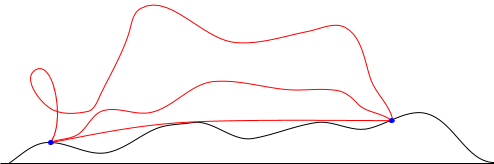
\includegraphics[width=.9\textwidth]{Principle_of_Least_Action_Variational_Methods/lagrangian_thing.png}
    \caption{A few different curves in the same class (beginning at the point $a$ and ending at $b$) constrained in a region of space.}
    \label{fig:my_label}
\end{figure}

We believe the particle should take the shortest and easiest possible path given the potential. But what does this mean?  In short, we wish to find the particle that, over the duration in time it is acting, uses the least amount of cost.
\end{ex}

\begin{ex}[The Minimal Surface]{ex: minimal_surf}
We can also consider a higher dimensional analog present in the study of (elastic) materials. \\

\emph{Consider a two-dimensional elastic membrane attached around its boundary to a wire subject to an external potential.  What shape does this membrane form?}\\

\begin{figure}[H]
    \centering
    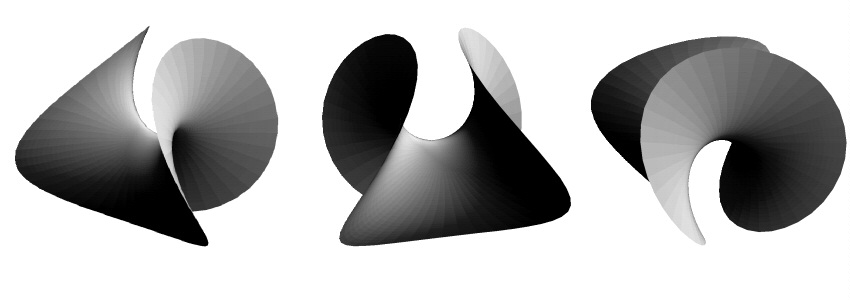
\includegraphics[width=.8\textwidth]{Principle_of_Least_Action_Variational_Methods/ennep.jpg}
    \caption{Enneper's surface. A minimal surface with boundary similar to the stitches on a baseball.}
    \label{fig:my_label}
\end{figure}

These membranes should use the least amount of area, as this stretching is not ideal for the elastic (it costs energy).  It turns out, this area and stretching are related to the curvature.
\end{ex}

\begin{df}[Action Functional]{def: action}
The \emph{action} functional $\mathcal{S}$ of a particle following a curve $\position \colon [0,1] \to \R^n$ is given by
\[
\action[\position]\coloneqq \int_0^1 \lagrangian dt.
\]
\end{df}



\begin{remark}
We want to provide the mathematical formulation of the \emph{least action} prinple.  Thus, we believe that we seek a minimizer for the action functional.
\end{remark}

\begin{ex}[The Popped Bubble]
I'm not totally sure that this example is correct and feasible, but it's worth of discussion at the very least.\\

\emph{Imagine a small bubble of an ideal gas in a large room. This gas is initially in a state given by the variables $P_0,V_0$, and $T_0$.  At time $t=0$ the bubble is popped and the gas is allowed to fill the room.  The final state is thus at some time, call it $t=1$, with a state defined by $P_1,V_1$, and $T_1$. How did the gas evolve between states?}\\

The goal would be to find the appropriate Lagrangian function and the associated action.  The trajectory in state space would then be the stationary point of this action.
\end{ex}

\section{The First Variation}

\subsection{Finite Dimensions}
When we seek to maximize a function $f\colon \R^n \to \R$, we first find stationary points.  A point $(x_1,\dots,x_n)$ is a \emph{stationary point} if it satisfies
\[
\nabla f(x_1,\dots,x_n)=\mathbf{0}.
\]
These are the points in which a function can attain a maximum or a minimum.  This is due to the fact that in an infinitesimal neighborhood of a stationary point, the function is essentially constant in each direction.

Our goal is to extend this notion to the infinite dimensional case, but we must define the correct notion of a functional derivative.

\subsection{Infinite Dimensions}

Let $V$ be an infinite dimensional real vector space equipped with a functional $\action \colon V \to R$.

\begin{df}[First Variation]{def: first_var}
The \emph{first variation of $\action$ in direction $v$} is
\[
\delta_v \action [u]\coloneqq \left.\frac{d}{d\epsilon} \action[u+\epsilon v]\right|_{\epsilon = 0},
\]
where $v$ is an element of the tangent space of $V$ at the point $u$, $T_uV$.
\end{df}

We think of this exactly like a directional derivative.  Based on this intuition, we say the following.

\begin{df}[Stationary Point]{def: stat_point}
If $\delta_v \action [u]=0$ for every $v\in T_uV$, then $u$ is a \emph{stationary point} of the functional $\action$.
\end{df}

We should now consider a few of the important cases.  Namely, we should investigate the Euler-Lagrange equations and the Laplace equation.

\begin{ex}[Euler-Lagrange Equations]{ex: e-l}
Let $V=(H^1([0,1]))^n$ (the trajectories in $\R^n$ with finite kinetic energy) and define
\[
\action[\position] = \int_{[0,1]} \lagrangian(\position,\velocity,t)dt.
\]
Then suppose that $\position$ is a stationary point of $\action$, i.e.
\[
\delta_v \action [\position] = 0, \quad\forall v \in T_{\position }V.
\]
Thus, we must have for all $v\in T_\position V$
\begin{align*}
    \left.\frac{d}{d\epsilon} \action [\position+\epsilon \mathbf{v}] \right|_{\epsilon=0}&=0\\
    \iff \left.\frac{d}{d\epsilon} \left(\int_{[0,1]} \lagrangian(\position + \epsilon \mathbf{v},\velocity + \epsilon \mathbf{\dot{v}},t)dt\right) \right|_{\epsilon=0}&=0\\
    \iff \int_{[0,1]} \left. \frac{d}{d\epsilon} \lagrangian(\position + \epsilon \mathbf{v},\velocity + \epsilon \mathbf{\dot{v}},t)\right|_{\epsilon=0} dt&=0\\
    \iff \int_{[0,1]} \frac{\partial \lagrangian}{\partial \position} \cdot \mathbf{v} + \frac{\partial \lagrangian}{\partial \velocity} \cdot \mathbf{\dot{v}}dt &=0.
\end{align*}
Now, we integrate by parts 
\[
\int_{[0,1]} \frac{\partial \lagrangian}{\partial \position}\cdot \mathbf{v} - \frac{d}{dt} \frac{\partial \lagrangian}{\partial \velocity} \cdot \mathbf{v} dt + \int_{\{0,1\}} \frac{\partial \lagrangian}{\partial \velocity} \cdot \mathbf{v}dt &=0
\]
and note that $T_{\position} V= (H_0^1([0,1]))^n$ means that
\[
\int_{\{0,1\}} \frac{\partial \lagrangian}{\partial \velocity} \cdot \mathbf{v}dt  =0.
\]
Thus we have that for all $v\in T_{\position} V$,
\[
\int_{[0,1]}\frac{\partial \lagrangian}{\partial \position}\cdot \mathbf{v} - \frac{d}{dt} \frac{\partial \lagrangian}{\partial \velocity} \cdot \mathbf{v} dt &=0.
\]
These are the \emph{weak Euler-Lagrange equations}. 

If our curve was in fact more regular, say $C^\infty$, then we get
\[
\frac{\partial \lagrangian}{\partial \position} - \frac{d}{dt} \frac{\partial \lagrangian}{\partial \velocity} = 0,
\]
which are the \emph{strong Euler-Lagrange equations.}
\end{ex}

\begin{prop}[Mechanical Least Action]{prop: mech_least_act}
The trajectory $\position$ of a particle is a stationary point of the action functional.\\

\noindent\emph{Proof.} Let $T(\velocity)=\frac{1}{2}m \langle \velocity, \velocity \rangle$ be the kinetic energy and $V(\position)$ be a potential. Then
\[
\lagrangian= T-V.
\]
So the Euler-Lagrange equations are then
\begin{align*}
    \frac{\partial \lagrangian}{\partial \position} - \frac{d}{dt} \frac{\partial \lagrangian}{\partial \velocity} &=0\\
    \iff -\frac{\partial V}{\partial \position} - \frac{d}{dt}\frac{\partial T}{\partial \velocity} &=0 \\
    -\nabla V |_{\position(t)} - \frac{d}{dt} \frac{\partial}{\partial \velocity} \frac{1}{2}m \langle \velocity,\velocity\rangle &=0 \\
    -\nabla V|_{\position(t)} - m \left.\frac{d}{dt} \velocity \right|_{\position(t)} &=0\\
    \iff -\nabla V |_{\position(t)}&=m\boldsymbol{\ddot{\gamma}}|_{\position(t)}.
\end{align*}
These are exactly Newton's laws if we consider a force from a potential
\[
\mathbf{F}=-\nabla V.
\]
\end{prop}


\begin{ex}[Laplace's Equation]{ex: laplace}
Let $\Omega\subset \R^n$ be open and consider $V=H^1(\Omega)$ and a functional $\action \colon V \to \R$ given by
\[
\action [u] = \int_\Omega \frac{1}{2} \|\nabla u\|^2 - fu.
\]
This action can be thought of as the Lagrangian for an elastic material being stressed under a force $f$. A critical point of this functional then satisfies
\[
\int_\Omega \nabla u \cdot \nabla v - fv = 0
\]
for all $v\in T_u V = H_0^1(\Omega)$.  This is the weak form of the Laplace equation.  The strong form then reads,
\[
-\Delta u = f
\]
and is obtained by integrating by parts.
\end{ex}

\section{Constrained Free Particles}

Instead of particles in $\R^n$, we can consider instead a particle confined to a Riemannian manifold $M$ with metric $\langle \cdot, \cdot \rangle$. We then can ask the following.

\begin{question}
For a free particle ($V=0$) with curve class $\position \colon [0,1] \to M$ with $p = \position(0)$ and $q=\position(1)$, which trajectory has the least action?
\end{question}

\begin{ex}[Geodesic Equations]{ex: geodesic}
To answer this question, consider the Lagrangian for a free particle that is solely the kinetic energy.  That is,
\[
\lagrangian = \frac{1}{2}m\langle \velocity, \velocity \rangle.
\]
Then the appropriate action 
\[
\action \colon \{\position \colon [0,1] \to M,~ \position(0)=p,~\position(1)=q\} \to \R
\]
is given by
\[
\action [\position] = \int_{[0,1]} \frac{1}{2}m\langle \velocity,\velocity \rangle dt.
\]

Let $x \colon M \to \R^n$ be local coordinates, define $\dot{x}^i = \frac{d}{dt}(x^i(\position(t)))$, and let $g_{ij}(x(\position(t)))$ be the local representation of the metric. Then the Euler-Lagrange equations reduce to 
\[
\ddot{x}^i(t)+\Gamma_{jk}^i (x(t))\dot{x}^j(t)\dot{x}^k(t)=0, \quad i=1,\dots,d,
\]
which are known as the \emph{geodesic equations.} Here, we have
\[
\Gamma_{jk}^i = \frac{1}{2}g^{i\ell} (g_{j\ell,k}+g_{k\ell,j}-g_{jk,\ell})
\]
where
\[
g_{i\ell,k}=\frac{\partial}{\partial x^k}g_{j\ell}.
\]
\end{ex}

\begin{remark}
What we have shown is that free particles naturally follow the geodesics on the space they are constrained to.
\end{remark}

\begin{question}
Can we consider every possible constrained situation as a particle situated on some manifold (possibly with boundary)?
\end{question}

\begin{ex}[Minimal Surface]{ex: min_surf}
\emph{Given a closed loop of wire and a soap film attached to this wire, what shape does the soap film take?}

We can phrase this problem in the following general way. Consider a Riemannian manifold $M$ and consider $N$ as a two-dimensional submanifold of $N$.  We can then define a volume on $N$ by pulling back the volume form $\eta$ on $M$ to $N$. This defines a volume functional on a class of submanifolds
\[
\textrm{Vol} \colon \{\Sigma ~\vert~ \textrm{$\Sigma$ 2-dimensional submanifold with $\partial \Sigma = \position$}\} \to \R.
\]
Given this volume form and the constraint that $\partial N$ is constrained to lie on a closed curve $\position$ in $M$, what manifold $N$ minimizes this volume functional?

It turns out that the critical point of this functional satisfies that the \emph{mean curvature} vanishes for all normal directions. This is rather intuitive as the curvature is akin to knowing about the stress of stretching on the membrane and we seek to minimize this stretching behavior.
\end{ex}

\end{document}